\documentclass[tikz,border=10pt]{standalone}
\usepackage{pgfplots}
\pgfplotsset{compat=newest}
\begin{document}
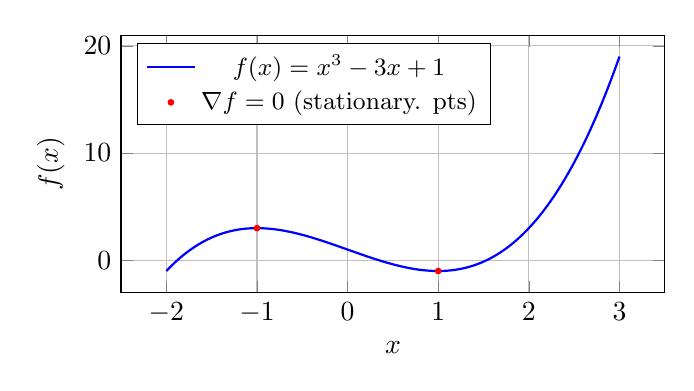
\begin{tikzpicture}
  \begin{axis}[
    width=0.7\textwidth,
    height=0.4\textwidth,
    xlabel={\(x\)},
    ylabel={\(f(x)\)},
    grid=both,
    domain=-2:3,
    samples=100,
    legend pos={north west},
    legend style={font=\small},
  ]
    \addplot[blue, thick] {x^3 - 3*x + 1};
    \addlegendentry{\(f(x) = x^3 - 3x + 1\)}
    \addplot[red, only marks, mark=*, mark size=1pt] coordinates {(-1, 3) (1, -1)};
    \addlegendentry{$\nabla f = 0$ (stationary. pts)}
  \end{axis}
\end{tikzpicture}
\end{document}
